% =============================================================================
%  DualPath: Quantifying the Cost of a Shared Memory Port
%  IEEE conference paper (IEEEtran, two-column).
%  Compile with pdfLaTeX (Overleaf default). Place the docs/diagrams/ and
%  docs/waveforms/ folders next to this file; any missing image is replaced by
%  a labelled placeholder so the paper always compiles.
% =============================================================================
\documentclass[conference]{IEEEtran}
\IEEEoverridecommandlockouts

\usepackage[T1]{fontenc}
\usepackage[utf8]{inputenc}
\usepackage{amsmath,amssymb,amsthm}
\usepackage{graphicx}
\graphicspath{{./}{diagrams/}{waveforms/}{docs/diagrams/}{docs/waveforms/}}
\usepackage{booktabs}
\usepackage{array}
\usepackage{tabularx}
\usepackage[table]{xcolor}
\usepackage[caption=false,font=footnotesize]{subfig}
\usepackage{algorithm}
\usepackage{algpseudocode}
\usepackage{listings}
\usepackage{tikz}
\usetikzlibrary{positioning,arrows.meta,calc,automata}
\usepackage{pgfplots}
\pgfplotsset{compat=1.17}
\usepackage{textcomp}
\usepackage{url}
\usepackage[hidelinks]{hyperref}
\usepackage[capitalise,nameinlink]{cleveref}

% ----------------------------------------------------------------------------
%  Theorem environments
% ----------------------------------------------------------------------------
\newtheorem{definition}{Definition}
\newtheorem{proposition}{Proposition}
\newtheorem{corollary}{Corollary}
\crefname{definition}{Definition}{Definitions}
\crefname{proposition}{Proposition}{Propositions}
\crefname{corollary}{Corollary}{Corollaries}
\crefname{lstlisting}{Listing}{Listings}
\crefname{algorithm}{Algorithm}{Algorithms}

% ----------------------------------------------------------------------------
%  Palette (matches the project's figures)
% ----------------------------------------------------------------------------
\definecolor{dpink}{HTML}{0F172A}
\definecolor{dpslate}{HTML}{64748B}
\definecolor{dpblue}{HTML}{2563EB}
\definecolor{dpgreen}{HTML}{16A34A}
\definecolor{dpred}{HTML}{DC2626}
\definecolor{dppurple}{HTML}{7C3AED}
\definecolor{dpbg}{HTML}{F1F5F9}

\lstset{
  language=Verilog, basicstyle=\ttfamily\scriptsize,
  keywordstyle=\color{dpblue}\bfseries, commentstyle=\color{dpslate}\itshape,
  backgroundcolor=\color{dpbg}, frame=none, xleftmargin=2pt,
  columns=fullflexible, keepspaces=true, showstringspaces=false,
  aboveskip=4pt, belowskip=2pt, captionpos=t,
  morekeywords={assign,wire,reg,always,posedge}
}

% ----------------------------------------------------------------------------
%  Macros
% ----------------------------------------------------------------------------
\newcommand{\NLS}{N_{\mathrm{LS}}}
\newcommand{\Tharv}{T_{\mathrm{H}}}
\newcommand{\Tshr}{T_{\mathrm{S}}}
\newcommand{\sig}[1]{\texttt{\detokenize{#1}}}
\newcommand{\safeimage}[2]{%
  \IfFileExists{#2}{\includegraphics[width=#1]{#2}}{%
    \fbox{\parbox[c][2.4cm][c]{0.95#1}{\centering\footnotesize
      Image \texttt{#2} not found: upload it next to \texttt{report.tex}.}}}}

% Timing-diagram helpers
\newcommand{\tdclk}[2]{%
  \foreach \c in {1,...,#2}{%
    \draw[dpink, line width=0.5pt] (\c-1,#1) -- (\c-1,#1+0.8) -- (\c-0.5,#1+0.8)
      -- (\c-0.5,#1) -- (\c,#1);}}
\newcommand{\tdbus}[5]{%
  \fill[fill=#5!14] (#2+0.08,#1) -- (#2,#1+0.4) -- (#2+0.08,#1+0.8) -- (#3-0.08,#1+0.8)
      -- (#3,#1+0.4) -- (#3-0.08,#1) -- cycle;
  \draw[draw=#5, line width=0.5pt] (#2+0.08,#1) -- (#2,#1+0.4) -- (#2+0.08,#1+0.8)
      -- (#3-0.08,#1+0.8) -- (#3,#1+0.4) -- (#3-0.08,#1) -- cycle;
  \node[font=\ttfamily\scriptsize] at ({(#2+#3)/2},#1+0.4) {#4};}
\newcommand{\tdhigh}[3]{%
  \fill[dpred!22] (#2,#1) rectangle (#3,#1+0.8);
  \draw[dpred, line width=0.7pt] (#2,#1) -- (#2,#1+0.8) -- (#3,#1+0.8) -- (#3,#1);}

% Float-only pages (the waveform page) start at the top instead of being centred.
\makeatletter
\setlength{\@fptop}{0pt}
\setlength{\@dblfptop}{0pt}
\setlength{\@dblfpsep}{12pt}
\makeatother
\renewcommand{\dbltopfraction}{0.9}
\renewcommand{\topfraction}{0.9}
\renewcommand{\textfraction}{0.07}

\begin{document}

\title{DualPath: The Cost of a Shared Memory Port\\in Harvard and von~Neumann Organizations}

\author{
\IEEEauthorblockN{Rajat Srivastav, Sachin, Anand, Rajdeep, and Omved Nagre}
\IEEEauthorblockA{Modern Computer Architecture, Capstone Project~9: Instruction and Data Memory Hierarchy\\
Source code and artifacts: \url{https://github.com/rajdeep-2004/dualpath}}
}

\maketitle

% =============================================================================
\begin{abstract}
A processor must fetch instructions and read or write data. Whether these two streams share one
memory port (the von~Neumann organization) or use separate paths (the Harvard organization)
decides whether an instruction and its operand can be accessed in the same clock cycle. This paper
implements a simplified Harvard memory organization, connects it to a simple processor, and
compares it with a shared-memory organization under controlled conditions. A 16-bit,
four-instruction, single-cycle processor is written once in Verilog-2001 and attached, without
modification, to two memory systems: a Harvard system with independent instruction and data
memories, and a shared system whose single-ported memory is arbitrated by a two-phase controller
that stalls the processor on every load or store. We derive a closed-form cycle model,
$\Tshr = \Tharv + \NLS$, which gives a cycles-per-instruction of $1+f$ for the shared system, where $f$
is the fraction of instructions that access data, and a throughput bound of $1/(1+f)$
instructions per cycle. We also identify and remove a combinational loop that arises when the
stall condition is taken from the processor's write enable. Three self-checking programs
reproduce the model exactly (5 versus 8, 4 versus 7, and 4 versus 4 cycles), and the simulation
waveforms show the Harvard system overlapping every load and store with its fetch while the
shared system serializes them.
\end{abstract}

\begin{IEEEkeywords}
Harvard architecture, von~Neumann architecture, structural hazard, memory organization,
address decoding, single-cycle processor, Verilog.
\end{IEEEkeywords}

% =============================================================================
\section{Introduction}
% =============================================================================

A stored-program processor retrieves two kinds of words from memory: the instructions it executes
and the data on which they operate. When both share one memory and one access path, the processor
cannot fetch an instruction and access its operand at the same time, and its throughput is limited
by that path. This limitation is widely known as the \emph{von~Neumann bottleneck}. The Harvard
organization removes the contention by giving the two streams independent storage and independent
access paths.

The difference between the two organizations is usually explained qualitatively: Harvard is
``faster'' because it can access instructions and data in parallel. This project asks how large
that difference is and exactly where it appears. Its objective is to implement a simplified
Harvard-style memory organization with separate instruction and data paths, connect it to a simple
processor, execute programs that contain both instruction fetches and data accesses, analyze the
opportunities for simultaneous access, and compare the result with a shared-memory organization.

To make the comparison fair, everything except the memory organization is held fixed: the same
processor, the same programs, and the same address map are used in both systems. The question
then becomes: \emph{how many clock cycles does a single shared memory port cost, and in which
cycles do they appear?} We answer it with a small but complete register-transfer-level (RTL)
design in which every signal can be inspected. The contributions are:
\begin{enumerate}
  \item A single-cycle processor with an explicit \emph{stall} input, attached unchanged to a
        Harvard memory system and to a single-ported shared memory system
        (\cref{sec:solution}).
  \item A two-phase port controller that decides when to stall from the fetched opcode, which
        avoids a combinational loop present in the straightforward design (\cref{sec:controller}).
  \item A closed-form cycle model and a throughput bound for both organizations
        (\cref{sec:model}).
  \item A self-checking verification environment whose measurements match the model exactly and
        whose waveforms show the mechanism cycle by cycle (\cref{sec:method,sec:results}).
\end{enumerate}

\Cref{sec:background} reviews the background, \cref{sec:solution} presents the design, the model,
and the experimental setup, \cref{sec:results} presents and discusses the results, and
\cref{sec:conclusion} concludes.

% =============================================================================
\section{Background}
\label{sec:background}
% =============================================================================

\subsection{Von~Neumann and Harvard Organizations}
In the stored-program machine described by von~Neumann, instructions and data reside in a single
memory. This makes programs easy to load and modify, and lets software decide how much memory is
used for code and how much for data. Its cost is contention: if the memory has one port, only one
access can complete per cycle, so an instruction fetch and a data access cannot overlap. The
Harvard organization, named after the Harvard Mark~I, keeps instructions and data in separate
memories, each with its own address and data lines. One fetch and one data access can then
complete in the same cycle, and a data store can never overwrite the program. \Cref{tab:orgs}
summarizes the properties that matter for this study.

\begin{table}[t]
\centering
\caption{The Two Organizations as Built in This Work}
\label{tab:orgs}
\footnotesize
\begin{tabularx}{\columnwidth}{@{}l X X@{}}
\toprule
 & \textbf{Shared (von~Neumann)} & \textbf{Harvard} \\
\midrule
Storage & One array for code and data & Separate arrays \\
Ports & One access per cycle & Two accesses per cycle \\
Load/store & Fetch, then data (stall) & Fetch and data together \\
Integrity & Stores may alter code & Stores cannot reach code \\
Flexibility & Code/data split by software & Split fixed in hardware \\
\bottomrule
\end{tabularx}
\end{table}

\subsection{Structural Hazards}
A structural hazard occurs when two operations need the same hardware resource in the same cycle.
A memory port that must serve both an instruction fetch and a data access is the standard example.
A processor can resolve it by stalling, or by duplicating the resource, which is what a Harvard
organization does. Modern processors combine both ideas: separate level-one instruction and data
caches (Harvard) in front of one shared main memory (von~Neumann), an arrangement known as the
\emph{modified Harvard} architecture. Microcontrollers often go further and keep program memory and
data memory physically separate.

\subsection{Why a Single-Cycle Processor}
The processor model decides whether the conflict is visible at all. A multi-cycle processor
already spends separate cycles on instruction fetch and memory access, so a shared memory can
serve both without any extra delay, and the two organizations take the same number of cycles. A
single-cycle processor needs the instruction and its operand within the same cycle. The port
conflict therefore appears directly as extra cycles, which makes the single-cycle processor the
smallest design in which the effect can be observed and measured.

\subsection{Scope of This Study}
In full systems, the benefit of separating instructions and data is mixed with cache hit rates,
memory latency, and pipelining, which makes it hard to isolate. This study removes those factors:
the memories have single-cycle access, the processor is not pipelined, and the memory organization
is the only variable that changes between the two systems.

% =============================================================================
\section{Proposed Solution}
\label{sec:solution}
% =============================================================================

This section describes the design, the analytical model, and the experimental setup. The design
contains every module the project calls for: a program counter, an instruction memory, a data
memory, an address decoder, and read/write control, together with a simple processor that uses
them. The processor is identical in both systems; only the memory side differs.

\subsection{Instruction Set}
The processor implements a 16-bit load/store instruction set (\cref{tab:isa}) with eight 16-bit
registers, \sig{R0} hard-wired to zero, and a 6-bit word-addressed space of 64 words. Data addresses
are computed as $(R[\mathit{rs1}] + \mathit{imm6}) \bmod 64$. Opcodes 4--15 are decoded as
\textsc{halt}. Because all memories are zero-initialized and \texttt{0x0000} encodes \textsc{halt},
execution beyond the end of a program terminates safely. \textsc{store} carries its value register
in bits 11--9 so that \emph{rs1} and \emph{imm6} occupy identical fields in both memory instructions,
which simplifies decoding.

\begin{table*}[t]
\centering
\caption{Instruction Set and 16-Bit Encoding}
\label{tab:isa}
\footnotesize
\begin{tabular}{@{}c l l c c c c@{}}
\toprule
Op & Mnemonic & Semantics & [15:12] & [11:9] & [8:6] & [5:0] \\
\midrule
0 & \textsc{halt} & stop; \sig{halted} $\leftarrow 1$, PC freezes & \texttt{0000} & \texttt{000} & \texttt{000} & \texttt{000000} \\
1 & \textsc{add} \emph{rd, rs1, rs2} & $R[rd] \leftarrow R[rs1] + R[rs2]$ & \texttt{0001} & \emph{rd} & \emph{rs1} & \emph{rs2}\,\texttt{000} \\
2 & \textsc{load} \emph{rd}, [\emph{rs1}+\emph{imm6}] & $R[rd] \leftarrow M[R[rs1]+imm6]$ & \texttt{0010} & \emph{rd} & \emph{rs1} & \emph{imm6} \\
3 & \textsc{store} \emph{rs2}, [\emph{rs1}+\emph{imm6}] & $M[R[rs1]+imm6] \leftarrow R[rs2]$ & \texttt{0011} & \emph{rs2} & \emph{rs1} & \emph{imm6} \\
\bottomrule
\end{tabular}
\end{table*}

\subsection{Datapath and Stall Interface}
Each instruction is fetched, decoded, executed, and written back within one clock cycle. The
register file provides two combinational read ports and one synchronous write port, and the program
counter advances by one word per completed instruction. A single signal,
\begin{equation}
  \mathit{run} = \overline{\mathit{stall}} \wedge \overline{\mathit{halted}},
  \label{eq:run}
\end{equation}
gates every architectural state change: the register write, the program-counter update, and the
memory write (\cref{lst:run}). When \sig{stall} is asserted, the instruction has no architectural
effect and is re-presented in the next cycle. This input is the \emph{only} interface difference
between the two systems.

\begin{lstlisting}[caption={Stall gating in the processor (\texttt{cpu.v}).},label={lst:run},float=t]
wire run = ~stall & ~halted_r;
// register write, PC update, memory write
.we(run & (is_add | is_load))  // register file
.en(run & ~is_halt)            // program counter
assign d_we = is_store & run;  // data memory
\end{lstlisting}

\subsection{Address Map and Decoding}
Both systems share the address map in \cref{tab:map}. A combinational decoder produces \sig{sel_mem},
\sig{sel_io}, and an error flag \sig{addr_err}. Because every instruction's bit fields drive some
value onto the address lines, \sig{addr_err} is qualified by a genuine access,
$\mathit{access} = \mathit{d\_re} \vee \mathit{d\_we}$, which prevents spurious errors during
arithmetic instructions. A read/write controller forwards the write enable only to the selected
target and multiplexes read data back to the processor. Address \texttt{0x3F} maps to an output
register.

\begin{table}[t]
\centering
\caption{Data Address Map (Both Systems)}
\label{tab:map}
\footnotesize
\begin{tabular}{@{}l l l@{}}
\toprule
Range & Target & Behaviour \\
\midrule
\texttt{0x00}--\texttt{0x0F} & memory & program area (shared system) \\
\texttt{0x10}--\texttt{0x2F} & memory & data area \\
\texttt{0x30}--\texttt{0x3E} & unmapped & \sig{addr_err}, write ignored, read 0 \\
\texttt{0x3F} & \sig{io_out} & memory-mapped output \\
\bottomrule
\end{tabular}
\end{table}

\begin{figure*}[t]
\centering
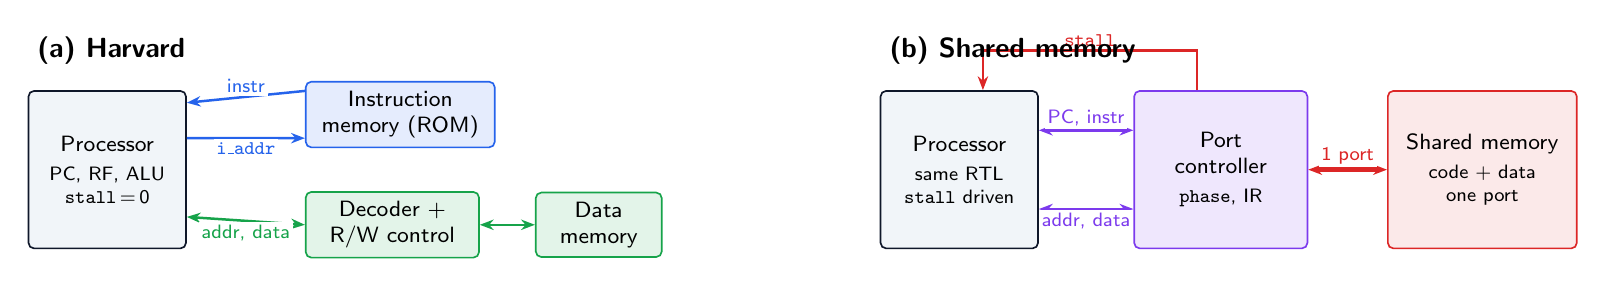
\begin{tikzpicture}[
  font=\sffamily\footnotesize, >={Stealth[length=5pt]},
  blk/.style={draw, rounded corners=2pt, align=center, line width=0.6pt, minimum height=8mm},
  cpu/.style={blk, fill=dpbg, draw=dpink, minimum width=20mm, minimum height=20mm},
  im/.style={blk, fill=dpblue!12, draw=dpblue, minimum width=24mm},
  dm/.style={blk, fill=dpgreen!12, draw=dpgreen, minimum width=22mm},
  sm/.style={blk, fill=dpred!10, draw=dpred, minimum width=24mm, minimum height=20mm},
  ct/.style={blk, fill=dppurple!12, draw=dppurple, minimum width=22mm, minimum height=20mm},
  lab/.style={font=\sffamily\scriptsize, fill=white, inner sep=1pt},
]
\node[cpu] (c1) {Processor\\[1pt]\scriptsize PC, RF, ALU\\[-1pt]\scriptsize \texttt{stall}\,=\,0};
\node[im, right=15mm of c1, yshift=7mm] (imem) {Instruction\\memory (ROM)};
\node[dm, right=15mm of c1, yshift=-7mm] (dec1) {Decoder +\\R/W control};
\node[dm, right=7mm of dec1, minimum width=16mm] (dmem) {Data\\memory};
\draw[->, dpblue, line width=0.9pt] ($(c1.east)+(0,4mm)$) -- node[lab, below]{\texttt{i\_addr}} ($(imem.west)+(0,-3mm)$);
\draw[->, dpblue, line width=0.9pt] ($(imem.west)+(0,3mm)$) -- node[lab, above]{instr} ($(c1.east)+(0,8.5mm)$);
\draw[<->, dpgreen, line width=0.9pt] ($(c1.east)+(0,-6mm)$) -- node[lab, below]{addr, data} (dec1.west);
\draw[<->, dpgreen, line width=0.9pt] (dec1) -- (dmem);
\node[font=\sffamily\bfseries, anchor=south west] at ($(c1.north west)+(0,2mm)$) {(a) Harvard};

\node[cpu, right=88mm of c1] (c2) {Processor\\[1pt]\scriptsize same RTL\\[-1pt]\scriptsize \texttt{stall} driven};
\node[ct, right=12mm of c2] (ctl) {Port\\controller\\[1pt]\scriptsize \texttt{phase}, IR};
\node[sm, right=10mm of ctl] (smem) {Shared memory\\[1pt]\scriptsize code + data\\[-1pt]\scriptsize one port};
\draw[<->, dppurple, line width=0.9pt] ($(c2.east)+(0,5mm)$) -- node[lab, above]{PC, instr} ($(ctl.west)+(0,5mm)$);
\draw[<->, dppurple, line width=0.9pt] ($(c2.east)+(0,-5mm)$) -- node[lab, below]{addr, data} ($(ctl.west)+(0,-5mm)$);
\draw[->, dpred, line width=0.9pt] ($(ctl.north)+(-3mm,0)$) -- ++(0,5mm) -| node[lab, pos=0.25, above]{\texttt{stall}} ($(c2.north)+(3mm,0)$);
\draw[<->, dpred, line width=1.6pt] (ctl) -- node[lab, above]{1 port} (smem);
\node[font=\sffamily\bfseries, anchor=south west] at ($(c2.north west)+(0,2mm)$) {(b) Shared memory};
\end{tikzpicture}
\caption{The two systems share one processor RTL. (a) Harvard: independent instruction (blue) and
data (green) paths; the processor is never stalled. (b) Shared: a two-phase controller multiplexes a
single memory port between fetch and data access and stalls the processor when both are required.
The decoder and output register of (a) are also present in (b) and are omitted for clarity.}
\label{fig:arch}
\end{figure*}

\subsection{Harvard System}
The Harvard system (\cref{fig:arch}a) connects the program counter to a $64\times16$ read-only
instruction memory and the data port. The data port passes through the decoder and read/write
controller to a $64\times16$ data memory and the output register. Both memories are read
combinationally, so an instruction and its operand are available within the same cycle, and the data
memory is written on the rising clock edge. Because the instruction memory exposes no write port,
instruction/data separation is a structural property rather than a software convention.

\subsection{Shared-Memory System}
\label{sec:controller}
The shared system stores code (\texttt{0x00}--\texttt{0x0F}) and data (\texttt{0x10}--\texttt{0x2F})
in one $64\times16$ array with exactly one port. A controller with a one-bit state \sig{phase} and a
16-bit instruction register \sig{IR} arbitrates the port (\cref{alg:ctrl,fig:fsm}). In the fetch phase
the port is addressed by the program counter. If the fetched word is a load or store, the controller
asserts \sig{stall}, latches the instruction into \sig{IR}, and enters the data phase. In the data
phase the port is addressed by the data address, the processor executes from \sig{IR}, and writes
are enabled.

\begin{algorithm}[t]
\caption{Port controller, one clock cycle}
\label{alg:ctrl}
\footnotesize
\begin{algorithmic}[1]
\If{$\mathit{phase}=0$} \Comment{fetch phase}
  \State $\mathit{addr} \gets \mathit{PC}$;\; $\mathit{instr} \gets M[\mathit{PC}]$
  \If{$\mathrm{op}(M[\mathit{PC}]) \in \{\textsc{load},\textsc{store}\}$}
    \State $\mathit{stall}\gets1$;\; $\mathit{IR}\gets M[\mathit{PC}]$;\; $\mathit{phase}\gets1$
  \Else
    \State $\mathit{stall}\gets0$ \Comment{instruction completes}
  \EndIf
\Else \Comment{data phase}
  \State $\mathit{addr}\gets\mathit{d\_addr}$;\; $\mathit{instr}\gets\mathit{IR}$; writes enabled
  \State $\mathit{stall}\gets0$;\; $\mathit{phase}\gets0$ \Comment{access completes}
\EndIf
\end{algorithmic}
\end{algorithm}

\begin{figure}[t]
\centering
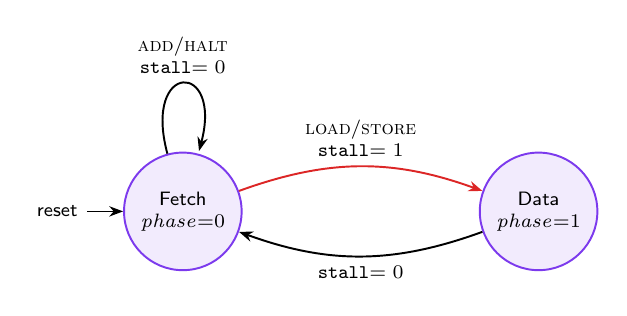
\begin{tikzpicture}[font=\sffamily\scriptsize, >={Stealth[length=5pt]}, node distance=30mm,
  every state/.style={draw=dppurple, fill=dppurple!10, line width=0.7pt, minimum size=14mm, align=center}]
\node[state, initial, initial text=reset] (F) {Fetch\\$\mathit{phase}{=}0$};
\node[state, right=of F] (D) {Data\\$\mathit{phase}{=}1$};
\path[->, line width=0.7pt]
 (F) edge[loop above] node[align=center]{\textsc{add}/\textsc{halt}\\ \texttt{stall}$=0$} (F)
 (F) edge[bend left=20, draw=dpred] node[above, align=center]{\textsc{load}/\textsc{store}\\ \texttt{stall}$=1$} (D)
 (D) edge[bend left=20] node[below, align=center]{\texttt{stall}$=0$} (F);
\end{tikzpicture}
\caption{Controller state machine. \texttt{stall} is a Mealy output that depends on the state and on
the opcode of the word read from memory.}
\label{fig:fsm}
\end{figure}

\textit{Avoiding a combinational loop.} A natural implementation asserts \sig{stall} whenever the
processor requests a data access ($\mathit{d\_re} \vee \mathit{d\_we}$). However, \eqref{eq:run}
forces $\mathit{d\_we}=0$ whenever $\mathit{stall}=1$, so \sig{stall} would depend combinationally
on \sig{d_we}, which in turn depends on \sig{stall}. For a store, the two signals have no stable
assignment. The controller instead decodes the opcode of the fetched word (\cref{lst:ctrl}), which
depends only on the memory output and the registered \sig{phase}. The loop is removed without
changing the intended behaviour.

\begin{lstlisting}[caption={Port arbitration (\texttt{shared\_mem\_controller.v}).},label={lst:ctrl},float=t]
wire op_ls = (mem_rdata[15:12] == 4'd2) ||
             (mem_rdata[15:12] == 4'd3);
assign stall    = ~phase & op_ls;
assign instr    = phase ? IR     : mem_rdata;
assign mem_addr = phase ? d_addr : pc;
assign mem_we   = phase & data_we;
\end{lstlisting}

\subsection{Analytical Model}
\label{sec:model}
\begin{definition}
A program executes a dynamic sequence of $N$ instructions, including the terminating \textsc{halt},
of which $\NLS$ are loads or stores. Its \emph{data-access fraction} is $f = \NLS/N \in [0,1)$. The
\emph{cycle count} $T$ of a system is the number of rising clock edges from reset release until
\sig{halted} is asserted, inclusive of \textsc{halt}.
\end{definition}

\begin{proposition}\label{prop:cycles}
For every program, $\Tharv = N$ and $\Tshr = N + \NLS$.
\end{proposition}

\begin{proof}
\emph{Harvard.} \sig{stall} is constant zero, so by \eqref{eq:run} every instruction completes in the
cycle in which it is fetched, giving $\Tharv = N$.
\emph{Shared.} Every instruction is first presented with $\mathit{phase}=0$, because reset initializes
the state to zero and both transitions of \cref{fig:fsm} return to it. An \textsc{add} or
\textsc{halt} completes in that cycle. A load or store asserts \sig{stall}, so by \eqref{eq:run} it
changes no architectural state. In the following cycle $\mathit{phase}=1$ and \sig{stall}$=0$, the
instruction completes from \sig{IR}, and the state returns to zero. Hence memory instructions cost
exactly two cycles and all others one, and $\Tshr = (N-\NLS) + 2\NLS = N + \NLS$.
\end{proof}

\begin{corollary}\label{cor:cpi}
$\mathrm{CPI}_{\mathrm{H}} = 1$, $\mathrm{CPI}_{\mathrm{S}} = 1+f$, and the speedup of the Harvard
organization is $S = \Tshr/\Tharv = 1+f$.
\end{corollary}

\textit{Port-demand bound.} Each instruction requires one fetch and, with probability $f$, one data
access, so a workload demands $1+f$ memory accesses per instruction. A single port supplies at most
one access per cycle, which bounds the shared system's throughput:
\begin{equation}
  \mathrm{IPC}_{\mathrm{S}} \le \frac{1}{1+f}, \qquad \mathrm{IPC}_{\mathrm{H}} = 1 .
  \label{eq:ipc}
\end{equation}
The controller attains the bound with equality, since the port is busy in every cycle.
\Cref{fig:ipc} plots \eqref{eq:ipc}. For a workload in which about a third of the instructions
access data ($f \approx 0.33$), a single shared port reduces throughput by about one quarter.

\begin{figure}[t]
\centering
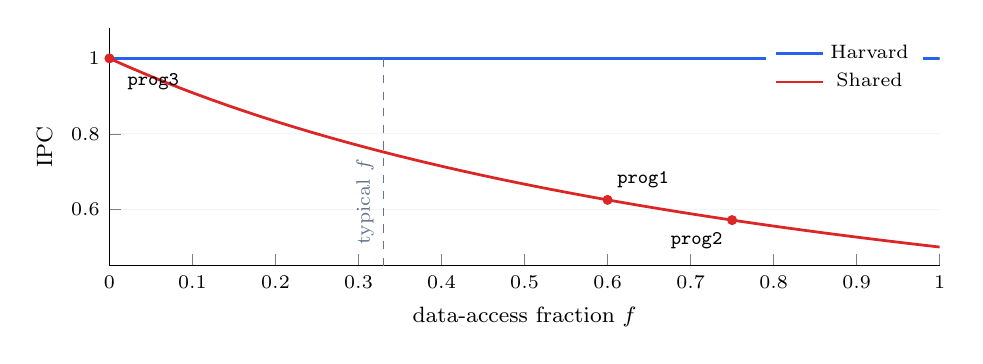
\begin{tikzpicture}
\begin{axis}[
  width=\columnwidth, height=4.6cm, xmin=0, xmax=1, ymin=0.45, ymax=1.08,
  xlabel={data-access fraction $f$}, ylabel={IPC},
  xlabel style={font=\footnotesize}, ylabel style={font=\footnotesize},
  tick label style={font=\scriptsize}, axis lines*=left, ymajorgrids, grid style={dpbg},
  legend style={draw=none, font=\scriptsize, at={(0.98,0.98)}, anchor=north east},
]
\addplot[dpblue, line width=1pt, domain=0:1] {1};
\addplot[dpred, line width=1pt, domain=0:1, samples=50] {1/(1+x)};
\addplot[only marks, mark=*, mark size=1.6pt, dpred] coordinates {(0,1) (0.6,0.625) (0.75,0.5714)};
\node[font=\scriptsize, anchor=south west] at (axis cs:0.6,0.63) {\texttt{prog1}};
\node[font=\scriptsize, anchor=north east] at (axis cs:0.75,0.565) {\texttt{prog2}};
\node[font=\scriptsize, anchor=north west] at (axis cs:0.01,0.985) {\texttt{prog3}};
\draw[dpslate, dashed] (axis cs:0.33,0.45) -- (axis cs:0.33,1.0);
\node[font=\scriptsize, dpslate, anchor=south, rotate=90] at (axis cs:0.33,0.62) {typical $f$};
\legend{Harvard, Shared}
\end{axis}
\end{tikzpicture}
\caption{Throughput as a function of the data-access fraction, from \eqref{eq:ipc}. Markers are the
measured values of the three workloads.}
\label{fig:ipc}
\end{figure}

\subsection{Experimental Setup and Verification}
\label{sec:method}
\textit{Implementation.} The design comprises twelve modules in synthesizable Verilog-2001
with synchronous active-high reset and no delay or simulation-only constructs in the RTL. Six modules
are shared by both systems (program counter, register file, processor, address decoder, read/write
controller, output register). The Harvard system adds instruction memory, data memory, and its top
level, and the shared system adds the shared memory, the port controller, and its top level.
Simulation uses Icarus Verilog~13.0 with all warnings enabled. Waveforms are recorded in VCD format
and inspected in the Surfer waveform viewer.

\textit{Workloads.} Three hand-encoded programs (\cref{tab:workloads}) exercise complementary
behaviour. \texttt{prog1} is the reference workload. \texttt{prog2} exercises address decoding,
including the output register and an unmapped address. \texttt{prog3} performs no data access and
serves as a control, for which \cref{prop:cycles} predicts identical cycle counts.

\begin{table}[t]
\centering
\caption{Workloads and Checked Properties}
\label{tab:workloads}
\footnotesize
\begin{tabularx}{\columnwidth}{@{}l >{\ttfamily}l X@{}}
\toprule
Prog. & \normalfont Machine code & Checked properties \\
\midrule
\texttt{prog1} & 2210 2411 1650 3620 0000 & R1\,=\,5, R2\,=\,7, R3\,=\,12, $M[\texttt{0x20}]$\,=\,12 \\
\texttt{prog2} & 2210 323F 3230 0000 & \sig{io_out}\,=\,5; \sig{addr_err} raised; $M[\texttt{0x30}], M[\texttt{0x3F}]$ unchanged \\
\texttt{prog3} & 1200 1448 1690 0000 & R1\,=\,R2\,=\,R3\,=\,0 (no data access) \\
\bottomrule
\end{tabularx}
\end{table}

\textit{Verification.} Each system has a self-checking testbench that applies reset, runs until
\sig{halted} (failing after 200 cycles), compares the final architectural state and cycle count with
expected values, and reports \textsc{pass} or \textsc{fail} with the precise mismatch. A single
command executes all six configurations, tabulates the results, and exits with an error if any check
fails.

\textit{Fault injection.} To confirm that the checks can fail, the adder was replaced by a subtractor.
The \texttt{prog1} testbench reported \texttt{R3: got 65534, expected 12}, and the comparison run
failed. A passing result therefore reflects correct behaviour rather than a vacuous test.

% =============================================================================
\section{Results and Discussion}
\label{sec:results}
% =============================================================================

\subsection{Cycle Counts}
All six configurations pass, and every measured cycle count equals the prediction of
\cref{prop:cycles} (\cref{tab:results,fig:bars}). The gap between the systems equals $\NLS$ for each
workload and vanishes for the control workload.

\begin{table}[t]
\centering
\caption{Measured Cycle Counts Versus the Model}
\label{tab:results}
\footnotesize
\begin{tabular}{@{}l c c c c c c@{}}
\toprule
Prog. & $N$ & $\NLS$ & $f$ & $\Tharv$ & $\Tshr$ (meas./model) & $S$ \\
\midrule
\texttt{prog1} & 5 & 3 & 0.60 & 5 & 8 / 8 & 1.60 \\
\texttt{prog2} & 4 & 3 & 0.75 & 4 & 7 / 7 & 1.75 \\
\texttt{prog3} & 4 & 0 & 0.00 & 4 & 4 / 4 & 1.00 \\
\bottomrule
\end{tabular}
\end{table}

\begin{figure}[t]
\centering
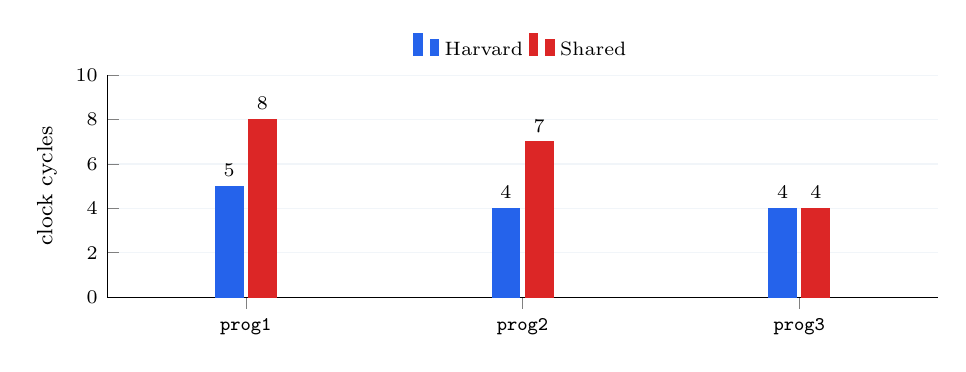
\begin{tikzpicture}
\begin{axis}[
  ybar, bar width=10pt, width=\columnwidth, height=4.4cm, ymin=0, ymax=10,
  ylabel={clock cycles}, ylabel style={font=\footnotesize},
  symbolic x coords={prog1,prog2,prog3}, xtick=data,
  xticklabel style={font=\ttfamily\scriptsize}, yticklabel style={font=\scriptsize},
  nodes near coords, nodes near coords style={font=\scriptsize},
  enlarge x limits=0.25, axis lines*=left, ymajorgrids, grid style={dpbg},
  legend style={draw=none, font=\scriptsize, at={(0.5,1.02)}, anchor=south, legend columns=2},
]
\addplot[fill=dpblue, draw=dpblue] coordinates {(prog1,5) (prog2,4) (prog3,4)};
\addplot[fill=dpred, draw=dpred] coordinates {(prog1,8) (prog2,7) (prog3,4)};
\legend{Harvard, Shared}
\end{axis}
\end{tikzpicture}
\caption{Cycles to completion for each workload.}
\label{fig:bars}
\end{figure}

\subsection{Timing Behaviour}
\Cref{fig:timing} reconstructs the execution of \texttt{prog1} from the simulation traces. In the
Harvard system, the instruction and data memories are both active in cycles 1, 2, and 4, so each
memory instruction performs its fetch and its data access in the same cycle. In the shared system,
the port is addressed by the program counter in cycle 1 while \sig{stall} is asserted, and by the
data address in cycle 2. The pattern repeats for every memory instruction, whereas the \textsc{add}
in cycle 5 completes without a stall. The captured waveforms (\cref{fig:waves}) display the same
behaviour directly.

\begin{figure*}[t]
\centering
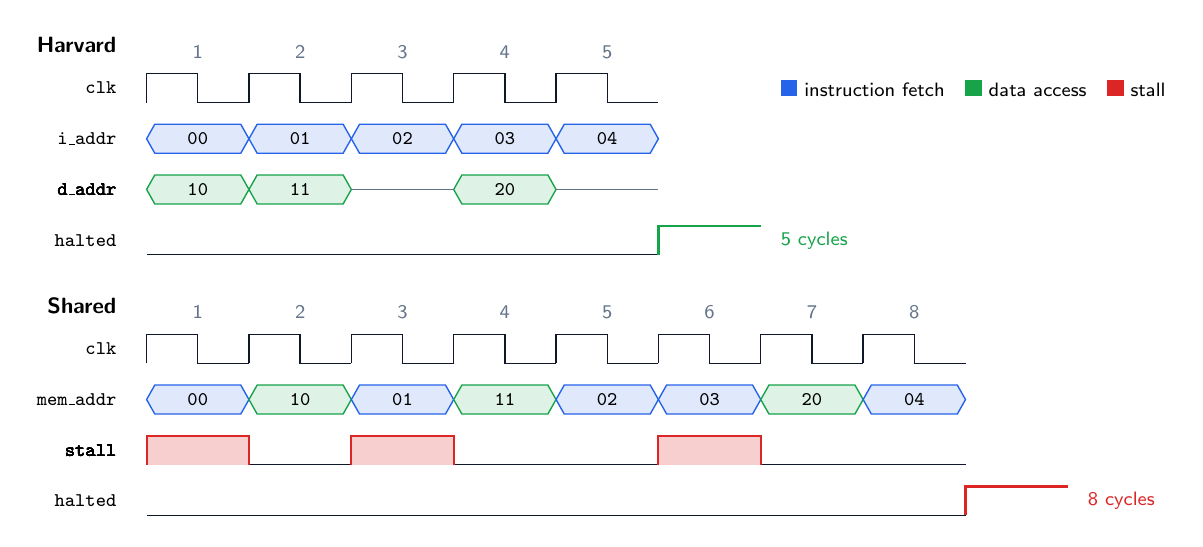
\begin{tikzpicture}[x=13mm, y=4.6mm, font=\sffamily\scriptsize]
  \node[anchor=east, font=\sffamily\bfseries\footnotesize] at (-0.2,11.6) {Harvard};
  \foreach \c in {1,...,5} \node[dpslate] at (\c-0.5,11.4) {\c};
  \node[anchor=east] at (-0.2,10.4) {\texttt{clk}};      \tdclk{10}{5}
  \node[anchor=east] at (-0.2,9.0)  {\texttt{i\_addr}};
     \foreach \c/\v in {1/00,2/01,3/02,4/03,5/04} \tdbus{8.6}{\c-1}{\c}{\v}{dpblue}
  \node[anchor=east] at (-0.2,7.6)  {\texttt{d\_addr}};
     \tdbus{7.2}{0}{1}{10}{dpgreen} \tdbus{7.2}{1}{2}{11}{dpgreen} \tdbus{7.2}{3}{4}{20}{dpgreen}
     \draw[dpslate, line width=0.4pt] (2,7.6) -- (3,7.6) (4,7.6) -- (5,7.6);
  \node[anchor=east] at (-0.2,6.2)  {\texttt{halted}};
     \draw[dpink, line width=0.5pt] (0,5.8) -- (5,5.8);
     \draw[dpgreen, line width=0.8pt] (5,5.8) -- (5,6.6) -- (6,6.6);
  \node[dpgreen, anchor=west] at (6.1,6.2) {5 cycles};

  \node[anchor=east, font=\sffamily\bfseries\footnotesize] at (-0.2,4.4) {Shared};
  \foreach \c in {1,...,8} \node[dpslate] at (\c-0.5,4.2) {\c};
  \node[anchor=east] at (-0.2,3.2) {\texttt{clk}};       \tdclk{2.8}{8}
  \node[anchor=east] at (-0.2,1.8) {\texttt{mem\_addr}};
     \foreach \c/\v/\k in {1/00/dpblue,2/10/dpgreen,3/01/dpblue,4/11/dpgreen,5/02/dpblue,6/03/dpblue,7/20/dpgreen,8/04/dpblue}
       \tdbus{1.4}{\c-1}{\c}{\v}{\k}
  \node[anchor=east] at (-0.2,0.4) {\texttt{stall}};
     \draw[dpink, line width=0.5pt] (0,0) -- (8,0);
     \tdhigh{0}{0}{1} \tdhigh{0}{2}{3} \tdhigh{0}{5}{6}
  \node[anchor=east] at (-0.2,-1.0) {\texttt{halted}};
     \draw[dpink, line width=0.5pt] (0,-1.4) -- (8,-1.4);
     \draw[dpred, line width=0.8pt] (8,-1.4) -- (8,-0.6) -- (9,-0.6);
  \node[dpred, anchor=west] at (9.1,-1.0) {8 cycles};

  \node[anchor=west] at (6.1,10.4) {\textcolor{dpblue}{\rule{6pt}{6pt}} instruction fetch\quad
     \textcolor{dpgreen}{\rule{6pt}{6pt}} data access\quad \textcolor{dpred}{\rule{6pt}{6pt}} stall};
\end{tikzpicture}
\caption{Cycle-level timing of \texttt{prog1} reconstructed from the simulation traces (values in
hexadecimal). The Harvard system overlaps fetch and data access in cycles 1, 2, and 4. The shared
port serves the program counter (blue) and then the data address (green) on consecutive cycles, with
\texttt{stall} asserted during each fetch of a load or store.}
\label{fig:timing}
\end{figure*}


\subsection{Memory Control and Separation}
\texttt{prog2} confirms the decoding behaviour in both systems. The store to \texttt{0x3F} reaches the
output register. The store to the unmapped address \texttt{0x30} raises \sig{addr_err} only during its
own data access and modifies no memory location. \sig{addr_err} remains deasserted in all other
cycles, including those of arithmetic instructions. In the Harvard system, no instruction sequence can
alter the program, because the instruction memory has no write port. In the shared system, a store to
\texttt{0x00}--\texttt{0x0F} would alter subsequent fetches.

\subsection{Interpretation}
Because the processor, workloads, and address map are held constant, the difference between the two
systems can be attributed only to the memory organization. The control workload confirms this by
producing identical cycle counts. The model is exact for this design because the controller adds
one cycle per memory instruction and none otherwise; equivalently, the single port is busy in every
cycle, so the shared system operates exactly at the bound of \eqref{eq:ipc}.

The same hazard appears in pipelined processors whenever a data access coincides with an
instruction fetch, and it is the reason modern processors use separate level-one instruction and
data caches in front of one shared main memory. These results quantify what that separation
recovers in the simplest case: a factor of $1+f$ in throughput, or about 30\% when a third of the
instructions access data. Because caches and pipelines change the balance in ways this model does
not capture, the figure is best read as the benefit of separation in a non-pipelined machine.

\subsection{Summary Against the Project Objectives}
\Cref{tab:objectives} maps each objective and evaluation criterion of the project to the evidence
presented in this paper.

\begin{table}[t]
\centering
\caption{Project Objectives and Supporting Evidence}
\label{tab:objectives}
\footnotesize
\begin{tabularx}{\columnwidth}{@{}>{\raggedright\arraybackslash}p{0.36\columnwidth} X@{}}
\toprule
Objective / criterion & Evidence \\
\midrule
Separate instruction and data paths & Harvard system (\cref{fig:arch}a); instruction memory has no write port \\
Connect to a simple processor & Single-cycle processor with stall input (\cref{tab:isa}, \cref{lst:run}) \\
Execute programs with fetches and data accesses & Three workloads, all checks pass (\cref{tab:workloads,tab:results}) \\
Memory control and address decoding & Decoder, read/write control, \sig{addr_err}, \sig{io_out} (\cref{tab:map}, \cref{fig:waves}c) \\
Timing behaviour & Cycle-level timing and waveforms (\cref{fig:timing,fig:waves}) \\
Simultaneous access opportunities & Fetch and data overlap in cycles 1, 2, 4 of \texttt{prog1} (\cref{fig:timing}) \\
Comparison with shared memory & Model and measurements: $\Tshr=\Tharv+\NLS$ (\cref{prop:cycles}, \cref{tab:results,fig:ipc}) \\
\bottomrule
\end{tabularx}
\end{table}

\subsection{Threats to Validity}
\textit{Idealized memories.} Memories are modelled as arrays with single-cycle, combinational read.
Synchronous SRAM or DRAM would add latency to both systems, but the relative cost of port contention
is unaffected under the assumptions of the model. \textit{Processor model.} The model applies to a
non-pipelined processor. In a pipeline, the cost also depends on scheduling and forwarding.
\textit{Workloads.} Three short programs exercise every datapath and control path but are not
representative of application behaviour. Without an immediate instruction, the control workload can
only produce zero values. \textit{Implementation.} The RTL follows synthesizable conventions but was
evaluated in simulation only, so clock frequency and area were not measured.

% Waveform figure: defined here so it lands at the top of the next page,
% above the end of the Conclusion and the Author Contributions.
\begin{figure*}[!t]
\centering
\subfloat[Harvard, \texttt{prog1}. \texttt{i\_addr}\,=\,\texttt{00} and \texttt{d\_addr}\,=\,\texttt{10} in the same cycle; \texttt{r3} becomes \texttt{000c} (12); \texttt{halted} rises after five cycles.]{%
  \safeimage{0.94\textwidth}{harvard-prog1-signals.png}}\\[6pt]
\subfloat[Shared memory, \texttt{prog1}. \texttt{mem\_addr} follows \texttt{00, 10, 01, 11, 02, 03, 20, 04}; \texttt{stall} is high for three cycles; \texttt{halted} rises after eight cycles.]{%
  \safeimage{0.94\textwidth}{shared-prog1-signals.png}}\\[6pt]
\subfloat[Harvard, \texttt{prog2}. The store to \texttt{0x3F} sets \texttt{io\_out}\,=\,5; the store to \texttt{0x30} raises \texttt{addr\_err} for one cycle and is discarded.]{%
  \safeimage{0.94\textwidth}{harvard-prog2-signals.png}}
\caption{Simulation waveforms captured in Surfer from the testbench output (values in hexadecimal).}
\label{fig:waves}
\end{figure*}
% =============================================================================
\section{Conclusion}
\label{sec:conclusion}
% =============================================================================
This project implemented a simplified Harvard memory organization with separate instruction and
data paths, connected it to a simple single-cycle processor, and compared it with a shared-memory
organization built around the same, unmodified processor. Analysis, simulation, and waveforms
agree. The Harvard organization sustains one instruction per cycle because every load and store
performs its fetch and its data access in the same cycle, and it enforces instruction/data
separation in hardware. The shared organization needs exactly one extra cycle per load or store,
$\Tshr = \Tharv + \NLS$, which gives $\mathrm{CPI}=1+f$. Future work could add branch and immediate
instructions for loop-based programs, synchronous memory models, separate caches in front of the
shared memory, a pipelined processor, and an FPGA implementation to measure frequency and area.

% =============================================================================
\section*{Author Contributions}
% =============================================================================
\noindent{\footnotesize
\begin{tabularx}{\columnwidth}{@{}l X@{}}
\toprule
Author & Contribution \\
\midrule
Rajat Srivastav & Register file and program counter \\
Sachin & Processor: instruction decode, control, address generation, and stall gating \\
Anand & Address decoder, read/write control, and memory-mapped output register \\
Rajdeep & Instruction and data memories, Harvard system integration, Harvard testbench, test programs, build flow, and documentation \\
Omved Nagre & Shared memory, port controller, shared system integration, and shared testbench \\
\bottomrule
\end{tabularx}}

\vspace{4pt}\noindent All authors contributed to the analysis of the results and approved the final manuscript.


\end{document}